\documentclass[aspectratio=169,11pt]{beamer}

% Theme and colors
\usetheme{Madrid}
\usecolortheme{whale}
\setbeamertemplate{navigation symbols}{}
\setbeamertemplate{footline}[frame number]

% Packages
\usepackage[utf8]{inputenc}
\usepackage[T1]{fontenc}
\usepackage{graphicx}
\usepackage{booktabs}
\usepackage{amsmath}
\usepackage{hyperref}
\usepackage{tikz}
\usetikzlibrary{shapes,arrows,positioning,calc}
\usepackage{siunitx}

% Bibliography
\usepackage[backend=biber,style=ieee,sorting=none]{biblatex}
\addbibresource{references.bib}

% Title information
\title[EECE5155 -- Module 2]{Engineering Project Characterization}
\subtitle{Module 2: From Problem to Specification -- Master's Level Rigor}
\author{Eduardo Baena}
\date{Spring 2026}
\institute{Northeastern University\\Department of Electrical and Computer Engineering\\
\texttt{e.baena@northeastern.edu}}

\begin{document}

% Title slide
\begin{frame}
    \titlepage
    \vspace{-1cm}
    \begin{center}
        \textbf{EECE5155: Wireless Sensor Networks and the Internet of Things}
    \end{center}
\end{frame}

% Learning Objectives
\begin{frame}{Learning Objectives}
    \textbf{By the end of this module, you should be able to:}
    
    \vspace{0.5cm}
    \begin{enumerate}
        \item \textbf{Distinguish} between a maker project and an engineering project
        \item \textbf{Characterize} a problem through systematic investigation
        \item \textbf{Document} design decisions with traceable justification
        \item \textbf{Verify} specifications against datasheets and literature
        \item \textbf{Defend} every number in your PES during oral examination
    \end{enumerate}
    
    \vspace{0.3cm}
    \begin{alertblock}{This is a Master's Program}
        Your PES is not a wish list. It is an \textbf{engineering document} that demonstrates research, understanding, and professional rigor.
    \end{alertblock}
\end{frame}

% Outline
\begin{frame}{Outline}
    \tableofcontents
\end{frame}

%==============================================================================
\section{Maker vs. Engineer: The Fundamental Difference}
%==============================================================================

\begin{frame}{What is a Maker Project?}
    \begin{columns}[T]
        \begin{column}{0.48\textwidth}
            \textbf{Maker approach:}
            \begin{itemize}
                \item ``I have an Arduino and some sensors''
                \item ``Let's see what I can build''
                \item ``It works on my desk''
                \item ``The tutorial said to use this''
                \item Copy-paste from Stack Overflow
                \item ``Good enough'' is the standard
            \end{itemize}
        \end{column}
        \begin{column}{0.48\textwidth}
            \textbf{Typical outcomes:}
            \begin{itemize}
                \item Works in demo, fails in deployment
                \item No understanding of failure modes
                \item Cannot explain design choices
                \item No documentation
                \item Not reproducible
                \item Not scalable
            \end{itemize}
        \end{column}
    \end{columns}
    
    \vspace{0.3cm}
    \begin{block}{The Problem}
        Maker projects are \textbf{exploratory}. They are valuable for learning, but they are \textbf{not engineering}.
    \end{block}
\end{frame}

\begin{frame}{What is an Engineering Project?}
    \begin{columns}[T]
        \begin{column}{0.48\textwidth}
            \textbf{Engineering approach:}
            \begin{itemize}
                \item Problem drives requirements
                \item Requirements drive design
                \item Design is \textbf{justified} and \textbf{documented}
                \item Every number has a \textbf{source}
                \item Failure modes are \textbf{analyzed}
                \item Testing \textbf{verifies} specifications
            \end{itemize}
        \end{column}
        \begin{column}{0.48\textwidth}
            \textbf{Expected outcomes:}
            \begin{itemize}
                \item Reproducible by another engineer
                \item Traceable decisions
                \item Known limitations
                \item Documented test results
                \item Defensible in review
                \item Scalable to production
            \end{itemize}
        \end{column}
    \end{columns}
    
    \vspace{0.3cm}
    \begin{alertblock}{Master's Level Expectation}
        You must be able to \textbf{defend every claim} in your document. ``I assumed'' or ``I guessed'' are not acceptable answers.
    \end{alertblock}
\end{frame}

\begin{frame}{The Difference in One Table}
    \begin{table}
        \centering
        \small
        \begin{tabular}{@{}p{3cm}p{5cm}p{5.5cm}@{}}
            \toprule
            \textbf{Aspect} & \textbf{Maker Project} & \textbf{Engineering Project} \\
            \midrule
            Sampling rate & ``1 Hz seems fine'' & ``Signal BW is X Hz (cite), Nyquist requires 2X, I use 2.5X'' \\
            \addlinespace
            Sensor choice & ``Amazon reviews'' & ``Datasheet: accuracy $\pm$0.5 C, meets req. R3'' \\
            \addlinespace
            Power estimate & ``Few months'' & ``Sleep: 2.1 uA (DS p.47), lifetime: 847 days'' \\
            \addlinespace
            Testing & ``Worked when I tried'' & ``N=50 samples, 95\% CI: [X, Y]'' \\
            \bottomrule
        \end{tabular}
    \end{table}
\end{frame}

%==============================================================================
\section{The Investigation Process}
%==============================================================================

\begin{frame}{Before You Write Anything: Research}
    \textbf{Your PES requires investigation, not assumptions.}
    
    \vspace{0.3cm}
    \begin{enumerate}
        \item \textbf{Literature review:} What has been done before?
        \begin{itemize}
            \item IEEE Xplore, Google Scholar, manufacturer white papers
            \item Minimum 5--10 relevant sources for your domain
        \end{itemize}
        
        \item \textbf{Domain expertise:} What do practitioners know?
        \begin{itemize}
            \item Industry standards (ISO, ASHRAE, FDA, etc.)
            \item Application notes from sensor manufacturers
        \end{itemize}
        
        \item \textbf{Physical characterization:} What are the actual constraints?
        \begin{itemize}
            \item Measure or cite: distances, temperatures, RF environment
            \item Do not guess deployment parameters
        \end{itemize}
    \end{enumerate}
    
    \vspace{0.3cm}
    \begin{block}{Example}
        ``Vaccine storage requires 2--8 C'' $\rightarrow$ \textbf{Source:} WHO PQS E006 specification
    \end{block}
\end{frame}

\begin{frame}{Sources of Engineering Data}
    \textbf{Where do your numbers come from?}
    
    \vspace{0.3cm}
    \begin{table}
        \centering
        \small
        \begin{tabular}{@{}p{3.5cm}p{4.5cm}p{4.5cm}@{}}
            \toprule
            \textbf{Parameter} & \textbf{Acceptable Source} & \textbf{Not Acceptable} \\
            \midrule
            Sensor accuracy & Manufacturer datasheet & ``Should be accurate'' \\
            \addlinespace
            Power consumption & Datasheet + measurement & Forum post, tutorial \\
            \addlinespace
            RF propagation & Published model + survey & ``WiFi works here'' \\
            \addlinespace
            Sampling rate & Signal analysis + Nyquist & ``1 Hz is common'' \\
            \addlinespace
            Protocol overhead & Specification document & ``About 20\%'' \\
            \bottomrule
        \end{tabular}
    \end{table}
    
    \vspace{0.3cm}
    \textbf{Rule:} Every number needs a citation or a measurement.
\end{frame}

\begin{frame}{Reading a Datasheet: What Engineers Extract}
    \textbf{Example: Temperature sensor selection}
    
    \vspace{0.3cm}
    \begin{columns}[T]
        \begin{column}{0.48\textwidth}
            \textbf{What a maker reads:}
            \begin{itemize}
                \item ``Measures temperature''
                \item ``Works with Arduino''
                \item ``\$3 on Amazon''
            \end{itemize}
            
            \vspace{0.3cm}
            \textbf{What an engineer extracts:}
            \begin{itemize}
                \item Accuracy: $\pm$0.5 C @ 25 C
                \item Resolution: 0.0625 C (12-bit)
                \item Response time: 750 ms (in oil)
                \item Operating range: -55 C to +125 C
                \item Supply current: 1 mA active
                \item Conversion time: 750 ms (12-bit)
            \end{itemize}
        \end{column}
        \begin{column}{0.48\textwidth}
            \textbf{Engineering questions:}
            \begin{itemize}
                \item Does accuracy meet my requirement?
                \item Is response time fast enough?
                \item What is power during conversion?
                \item How does accuracy degrade at extremes?
                \item What is the interface timing?
            \end{itemize}
            
            \vspace{0.3cm}
            \textbf{Your PES must answer these.}
        \end{column}
    \end{columns}
\end{frame}

%==============================================================================
\section{Problem Characterization}
%==============================================================================

\begin{frame}{Problem Definition: The Foundation}
    \textbf{A well-defined problem is half the solution.}
    
    \vspace{0.3cm}
    \begin{alertblock}{Bad Problem Statement}
        ``Monitor temperature in a building to improve energy efficiency.''
        
        $\rightarrow$ What building? What temperature? What efficiency metric?
    \end{alertblock}
    
    \vspace{0.3cm}
    \begin{exampleblock}{Good Problem Statement}
        ``HVAC in Snell Engineering consumes 2.1 GWh/year. Zone-level temperature monitoring (currently absent) could enable demand-controlled ventilation, reducing consumption by 15--25\% (DOE estimate). This project implements a 50-node WSN for 5-minute resolution data across 12 zones.''
    \end{exampleblock}
    
    \vspace{0.2cm}
    \textbf{Notice:} Specific location, quantified baseline, cited estimate, defined scope.
\end{frame}

\begin{frame}{Baseline: What Exists Today?}
    \textbf{You cannot improve what you do not measure.}
    
    \vspace{0.3cm}
    \begin{columns}[T]
        \begin{column}{0.48\textwidth}
            \textbf{Questions to answer:}
            \begin{itemize}
                \item How is this done today?
                \item What are the current costs?
                \item What are the failure modes?
                \item Who are the stakeholders?
                \item What data exists already?
            \end{itemize}
        \end{column}
        \begin{column}{0.48\textwidth}
            \textbf{How to find out:}
            \begin{itemize}
                \item Interview domain experts
                \item Review existing systems
                \item Analyze historical data
                \item Read industry reports
                \item Conduct site surveys
            \end{itemize}
        \end{column}
    \end{columns}
    
    \vspace{0.3cm}
    \begin{block}{Example}
        ``Current: Manual logging 2x/day. Failure rate: 3 excursions/month detected after 4+ hours. Cost: \$12,000/year spoiled inventory (facility records, 2024).''
    \end{block}
\end{frame}

\begin{frame}{Alternatives Analysis: Why Your Approach?}
    \textbf{Engineering requires considering alternatives.}
    
    \vspace{0.3cm}
    \begin{table}
        \centering
        \small
        \begin{tabular}{@{}p{2.5cm}p{4.5cm}p{5.5cm}@{}}
            \toprule
            \textbf{Alternative} & \textbf{Analysis} & \textbf{Rejection Rationale} \\
            \midrule
            Wired sensors & Lower power, reliable & Install cost \$150/point $\times$ 50 = \$7,500 \\
            \addlinespace
            Commercial & Proven, supported & \$89/sensor + \$29/mo = \$2,200/yr \\
            \addlinespace
            BLE mesh & Low power & Range 10m; needs 15+ repeaters \\
            \addlinespace
            LoRaWAN & Long range, low power & \textbf{Selected:} \$800 total BOM \\
            \bottomrule
        \end{tabular}
    \end{table}
    
    \vspace{0.2cm}
    \textbf{Notice:} Quantified comparison, not opinions.
\end{frame}

%==============================================================================
\section{Signal Characterization}
%==============================================================================

\begin{frame}{What Are You Actually Measuring?}
    \textbf{Signal characterization requires understanding the physics.}
    
    \vspace{0.3cm}
    \begin{columns}[T]
        \begin{column}{0.48\textwidth}
            \textbf{Questions to answer:}
            \begin{itemize}
                \item What is the physical phenomenon?
                \item What is the expected range?
                \item What is the signal bandwidth?
                \item What accuracy is required?
                \item What is the noise environment?
            \end{itemize}
        \end{column}
        \begin{column}{0.48\textwidth}
            \textbf{How to determine:}
            \begin{itemize}
                \item Physics/domain literature
                \item Preliminary measurements
                \item Industry standards
                \item Application requirements
                \item Site characterization
            \end{itemize}
        \end{column}
    \end{columns}
    
    \vspace{0.3cm}
    \begin{alertblock}{Common Failure}
        ``I'll sample at 1 kHz to be safe.'' $\rightarrow$ \textbf{Why?} What is the signal bandwidth? This wastes power and storage without justification.
    \end{alertblock}
\end{frame}

\begin{frame}{Sampling Rate: Engineering Justification}
    \textbf{Nyquist is necessary but not sufficient.}
    
    \vspace{0.3cm}
    \textbf{Process:}
    \begin{enumerate}
        \item \textbf{Determine signal bandwidth} from physics or measurement
        \item \textbf{Apply Nyquist:} $f_s > 2 f_{max}$
        \item \textbf{Add margin} for anti-aliasing (typically 2.5--4$\times$)
        \item \textbf{Consider application:} detection latency, event capture
        \item \textbf{Document the reasoning}
    \end{enumerate}
    
    \vspace{0.3cm}
    \begin{exampleblock}{Example: Room Temperature}
        Thermal time constant: $\tau \approx$ 20 min $\rightarrow$ $f_{3dB} \approx 0.0001$ Hz\\
        Nyquist minimum: 1 sample / 83 min\\
        Application requirement: 5-min resolution for HVAC control\\
        \textbf{Selected:} 1 sample / 5 min (application-driven, exceeds Nyquist)
    \end{exampleblock}
\end{frame}

\begin{frame}{Resolution vs. Accuracy: Not the Same}
    \textbf{A common confusion that reveals lack of understanding.}
    
    \vspace{0.3cm}
    \begin{columns}[T]
        \begin{column}{0.48\textwidth}
            \textbf{Resolution:}
            \begin{itemize}
                \item Smallest detectable change
                \item Determined by ADC bits
                \item Example: 12-bit, 3.3V range
                \item Resolution = 0.8 mV
            \end{itemize}
        \end{column}
        \begin{column}{0.48\textwidth}
            \textbf{Accuracy:}
            \begin{itemize}
                \item Closeness to true value
                \item Includes all error sources
                \item Example: $\pm$2\% of reading
                \item At 25 C: $\pm$0.5 C
            \end{itemize}
        \end{column}
    \end{columns}
    
    \vspace{0.3cm}
    \begin{alertblock}{Engineering Question}
        ``My sensor has 16-bit resolution. Is it accurate?''
        
        $\rightarrow$ \textbf{No.} Resolution $\neq$ accuracy. A 16-bit ADC with noise and poor calibration can be worse than a well-designed 8-bit system.
    \end{alertblock}
\end{frame}

%==============================================================================
\section{Constraint Analysis and Tradeoffs}
%==============================================================================

\begin{frame}{Constraints Must Be Quantified}
    \textbf{``Low power'' is not a constraint. ``$<$50 $\mu$A average'' is.}
    
    \vspace{0.3cm}
    \begin{table}
        \centering
        \small
        \begin{tabular}{@{}p{2.5cm}p{2.5cm}p{7cm}@{}}
            \toprule
            \textbf{Constraint} & \textbf{Target} & \textbf{Derivation} \\
            \midrule
            Battery life & $>$2 years & Maintenance cycle; site visit cost \$200 \\
            \addlinespace
            Avg current & $<$47 $\mu$A & 2000 mAh / 2 years / 8760 h \\
            \addlinespace
            Latency & $<$5 min & HVAC control loop requirement \\
            \addlinespace
            Range & $>$50 m & Building dimension + margin (survey) \\
            \addlinespace
            Cost/node & $<$\$30 & 50 nodes $\times$ \$30 = \$1500 budget \\
            \bottomrule
        \end{tabular}
    \end{table}
    
    \vspace{0.2cm}
    \textbf{Notice:} Each target has a derivation you can defend.
\end{frame}

\begin{frame}{Power Budget: Show Your Work}
    \textbf{This is where maker projects fail.}
    
    \vspace{0.2cm}
    \begin{table}
        \centering
        \footnotesize
        \begin{tabular}{@{}p{3.5cm}p{2cm}p{2cm}p{2cm}p{2.5cm}@{}}
            \toprule
            \textbf{State} & \textbf{Current} & \textbf{Duration} & \textbf{Period} & \textbf{Avg Contrib.} \\
            \midrule
            Deep sleep & 2.1 $\mu$A & 299.2 s & 300 s & 2.09 $\mu$A \\
            Wake + sensor & 8 mA & 100 ms & 300 s & 2.67 $\mu$A \\
            Radio TX & 120 mA & 50 ms & 300 s & 20.0 $\mu$A \\
            Radio RX window & 12 mA & 500 ms & 300 s & 20.0 $\mu$A \\
            Processing & 6 mA & 50 ms & 300 s & 1.0 $\mu$A \\
            \midrule
            \textbf{Total average} & & & & \textbf{45.8 $\mu$A} \\
            \bottomrule
        \end{tabular}
    \end{table}
    
    \vspace{0.2cm}
    \textbf{Sources:} Sleep: STM32L072 DS Table 25. Radio: SX1276 DS Table 7.
    
    \textbf{Lifetime:} 2000 mAh / 45.8 $\mu$A = 43,668 h = \textbf{4.98 years}
\end{frame}

\begin{frame}{Tradeoff Documentation}
    \textbf{Engineering is about tradeoffs. Document them.}
    
    \vspace{0.3cm}
    \begin{exampleblock}{Example: Sampling Rate vs. Battery Life}
        \textbf{Options analyzed:}
        \begin{itemize}
            \item 1 sample/min: 45.8 $\mu$A, 4.98 yr life, 5-min latency OK
            \item 1 sample/5min: 12.3 $\mu$A, 18.5 yr life, 10-min latency marginal
            \item 1 sample/10s: 267 $\mu$A, 0.85 yr life, excellent latency
        \end{itemize}
        
        \textbf{Decision:} 1 sample/min selected.
        
        \textbf{Rationale:} Meets 2-year requirement with 2.5$\times$ margin. 5-min latency acceptable for HVAC (response $>$15 min).
    \end{exampleblock}
    
    \vspace{0.2cm}
    \textbf{This is the level of documentation expected.}
\end{frame}

%==============================================================================
\section{Verification and Testing}
%==============================================================================

\begin{frame}{Testing is Not Optional}
    \textbf{``It works'' is not verification.}
    
    \vspace{0.3cm}
    \begin{columns}[T]
        \begin{column}{0.48\textwidth}
            \textbf{What must be tested:}
            \begin{itemize}
                \item Sensor accuracy (vs. reference)
                \item Power consumption (measured)
                \item RF range (site survey)
                \item Packet delivery rate
                \item Environmental limits
                \item Long-term stability
            \end{itemize}
        \end{column}
        \begin{column}{0.48\textwidth}
            \textbf{How to document:}
            \begin{itemize}
                \item Test procedure (reproducible)
                \item Equipment used (calibrated?)
                \item Sample size (N $\geq$ 30)
                \item Results with uncertainty
                \item Pass/fail vs. requirement
            \end{itemize}
        \end{column}
    \end{columns}
    
    \vspace{0.3cm}
    \begin{alertblock}{Master's Level Expectation}
        Your final report must include test results that \textbf{verify} your specifications. ``I didn't have time'' is a failing grade.
    \end{alertblock}
\end{frame}

\begin{frame}{Example: Power Measurement}
    \textbf{How to verify your power budget:}
    
    \vspace{0.3cm}
    \begin{enumerate}
        \item \textbf{Equipment:} Current meter with $\mu$A resolution (Nordic PPK2)
        \item \textbf{Procedure:}
        \begin{itemize}
            \item Measure sleep current for 60 s (verify stability)
            \item Capture 10 complete wake/TX/sleep cycles
            \item Calculate average current over full period
        \end{itemize}
        \item \textbf{Results:}
        \begin{itemize}
            \item Measured sleep: 2.3 $\mu$A (spec: 2.1) -- 10\% higher
            \item Measured TX: 125 mA (spec: 120) -- 4\% higher
            \item Measured avg: 48.2 $\mu$A (calc: 45.8) -- 5\% higher
        \end{itemize}
        \item \textbf{Conclusion:} Within 10\% of calculated. Revised lifetime: 4.7 years. Still exceeds 2-year requirement.
    \end{enumerate}
\end{frame}

\begin{frame}{RF Site Survey: Not Optional}
    \textbf{``WiFi works here'' is not RF characterization.}
    
    \vspace{0.3cm}
    \textbf{What you must measure or model:}
    \begin{itemize}
        \item Path loss at your frequency (915 MHz $\neq$ 2.4 GHz)
        \item Wall attenuation (concrete: 10--15 dB, drywall: 3--5 dB)
        \item Multipath and fading margin (typically 10--20 dB)
        \item Interference sources (other radios, motors, etc.)
    \end{itemize}
    
    \vspace{0.3cm}
    \begin{exampleblock}{Link Budget Example}
        TX power: +14 dBm\\
        Path loss (50m indoor): -75 dB (log-distance model, n=3.5)\\
        Wall loss (2 concrete): -24 dB\\
        Fading margin: -15 dB\\
        RX sensitivity: -137 dBm (LoRa SF12)\\
        \textbf{Link margin:} +14 - 75 - 24 - 15 - (-137) = \textbf{+37 dB} (OK)
    \end{exampleblock}
\end{frame}

%==============================================================================
\section{Documentation Standards}
%==============================================================================

\begin{frame}{What Your PES Must Contain}
    \textbf{Every section requires:}
    
    \vspace{0.3cm}
    \begin{enumerate}
        \item \textbf{Claim:} What you are stating
        \item \textbf{Evidence:} Data, measurement, or citation
        \item \textbf{Reasoning:} Why this evidence supports the claim
        \item \textbf{Traceability:} Where to find the source
    \end{enumerate}
    
    \vspace{0.3cm}
    \begin{exampleblock}{Example}
        \textbf{Claim:} Sampling rate of 1 sample/5 min is sufficient.\\
        \textbf{Evidence:} Room thermal time constant is 15--30 min (ASHRAE Handbook, Ch. 18).\\
        \textbf{Reasoning:} Signal bandwidth $<$0.001 Hz; Nyquist requires $>$1 sample/8 min; 1/5 min provides 60\% margin.\\
        \textbf{Traceability:} ASHRAE Fundamentals 2021, Chapter 18, Table 4.
    \end{exampleblock}
\end{frame}

\begin{frame}{Common Failures That Will Cost You Points}
    \begin{alertblock}{Avoid These}
        \begin{enumerate}
            \item \textbf{Vague problem:} ``Improve efficiency'' $\rightarrow$ What? By how much?
            
            \item \textbf{No baseline:} ``Monitor X'' $\rightarrow$ How is it done today?
            
            \item \textbf{Missing units:} ``Sample at 100'' $\rightarrow$ 100 what?
            
            \item \textbf{No source:} ``Accuracy is 1\%'' $\rightarrow$ Says who? Datasheet page?
            
            \item \textbf{Assumed parameters:} ``Range is 50m'' $\rightarrow$ Did you measure?
            
            \item \textbf{No error analysis:} ``Power is 45 $\mu$A'' $\rightarrow$ Uncertainty? Conditions?
            
            \item \textbf{Untested claims:} ``Will work for 2 years'' $\rightarrow$ How do you know?
        \end{enumerate}
    \end{alertblock}
\end{frame}

\begin{frame}{The Oral Defense}
    \textbf{You will be asked to defend your PES.}
    
    \vspace{0.3cm}
    \textbf{Questions you must be able to answer:}
    \begin{itemize}
        \item ``Why did you choose this sampling rate?''
        \item ``Where does this power number come from?''
        \item ``What happens if your assumption X is wrong?''
        \item ``How did you verify this specification?''
        \item ``What alternatives did you consider?''
        \item ``What is the uncertainty in this measurement?''
    \end{itemize}
    
    \vspace{0.3cm}
    \begin{alertblock}{Unacceptable Answers}
        ``I assumed...'' / ``I guessed...'' / ``The tutorial said...'' / ``It seemed reasonable...'' / ``I didn't have time to measure...''
    \end{alertblock}
\end{frame}

%==============================================================================
\section{Connecting to Module 3}
%==============================================================================

\begin{frame}{From Specification to Processing}
    \begin{center}
    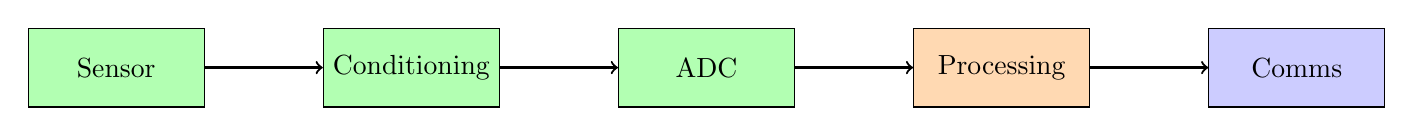
\begin{tikzpicture}[node distance=1.5cm, auto,
        block/.style={rectangle, draw, fill=blue!20, text width=2cm, text centered, minimum height=1cm},
        done/.style={rectangle, draw, fill=green!30, text width=2cm, text centered, minimum height=1cm},
        next/.style={rectangle, draw, fill=orange!30, text width=2cm, text centered, minimum height=1cm}]
        
        \node[done] (sensor) {Sensor};
        \node[done, right=of sensor] (cond) {Conditioning};
        \node[done, right=of cond] (adc) {ADC};
        \node[next, right=of adc] (proc) {Processing};
        \node[block, right=of proc] (comm) {Comms};
        
        \draw[->, thick] (sensor) -- (cond);
        \draw[->, thick] (cond) -- (adc);
        \draw[->, thick] (adc) -- (proc);
        \draw[->, thick] (proc) -- (comm);
    \end{tikzpicture}
    \end{center}
    
    \vspace{0.3cm}
    \textbf{Your PES constraints drive MCU selection:}
    \begin{itemize}
        \item Power budget $\rightarrow$ Sleep current, active current
        \item Processing needs $\rightarrow$ CPU speed, memory
        \item Interface requirements $\rightarrow$ Peripherals (SPI, I2C, ADC)
        \item Cost target $\rightarrow$ MCU price point
    \end{itemize}
    
    \vspace{0.2cm}
    \textbf{Module 3} will cover computing architectures and how to select the right platform.
\end{frame}

%==============================================================================
\section{Summary}
%==============================================================================

\begin{frame}{Module Summary}
    \textbf{Key Takeaways:}
    
    \vspace{0.3cm}
    \begin{enumerate}
        \item \textbf{Engineering $\neq$ Making:} Every decision must be justified and documented
        \item \textbf{Research first:} Literature, datasheets, standards, measurements
        \item \textbf{Quantify everything:} Numbers with units, sources, and uncertainty
        \item \textbf{Document tradeoffs:} Show alternatives considered and why rejected
        \item \textbf{Verify specifications:} Test results, not assumptions
        \item \textbf{Be defensible:} You will explain every number in your PES
    \end{enumerate}
    
    \vspace{0.3cm}
    \begin{block}{Your Task}
        Start your PES with this rigor. Every section should demonstrate investigation, understanding, and professional engineering practice.
    \end{block}
\end{frame}

\begin{frame}{Questions?}
    \begin{center}
        \Large
        \textbf{Questions?}
        
        \vspace{1cm}
        \normalsize
        \textbf{Next:} Module 3 -- Local Data Processing
        
        \vspace{0.5cm}
        Computing architectures, MCU selection, power/performance tradeoffs
    \end{center}
\end{frame}

%==============================================================================
% References
%==============================================================================

\begin{frame}[allowframebreaks]{References}
    \printbibliography
\end{frame}

\end{document}
